\svnid{$Id: highlevel.tex 74563 2022-02-13 20:35:17Z jagers $}

\chapter{High level routines} \label{Chp:HighLevelRoutines}
Although the low level routines provide access to all data in the NEFIS files, obtaining a useful, consistent data set can be difficult.
For instance, to plot a 2D vector field you have to combine the information stored at about seven locations in the Delft3D communication file.
Therefore, a number of high level routines has been provided to simplify the plotting and data retrieval operations.
Routines are provided for plotting a grid (with grid number labels), plotting thin dams and inactive velocity points, and retrieving data to plot velocity vectors.
Functions are also provided for reading and writing \DRGFGRID\  grid files (\DRGFGRID\  manual~\citep{RGF_UM}), \DQUICKIN\ depth files (\DQUICKIN\ manual~\citep{QUICKIN_UM}, and \DFLOW\ restart files (\DFLOW\ manual~\citep{FLOW_UM}).

\section{Plot a grid: \command{drawgrid}}

\subsection*{Purpose}
Plot the morphological grid.

\subsection*{Syntax}
\begin{Verbatim}
drawgrid(NFStruct)
[X, Y] = drawgrid(NFStruct);
drawgrid(X, Y)
\end{Verbatim}

\subsection*{Description}
\command{drawgrid(NFStruct)} where \command{NFStruct} is the structure obtained from the \vsuse\ command.
The function adds the morphological grid (that is, the user-defined grid) to the current axes.
\file{trim-$\ast$}, \file{tram-$\ast$}, \file{botm-$\ast$}, and \file{com-$\ast$} files are supported.
The morphological grid equals the grid specified in the input file; the bed level points are specified on the grid line crossings.

\command{[X, Y] = drawgrid(NFStruct)} returns the X and Y co-ordinates, but it does not actually draw the morphological grid.

\command{drawgrid(X, Y)} draws the user specified grid in the current axes.

This function accepts a number of optional arguments, which consist of property - value pairs similar to those use by the MATLAB \command{set} command:
\command{drawgrid(..., 'optionname1', optionval1, 'optionname2', optionval2, ...)}.
The supported options are

\begin{guilist}
\item['color'] The value can be an RGB-triplet, a colour character ('r', 'g', 'b', 'c', 'm', 'y', 'k', 'w'), or the string 'ortho' for colouring based on the orthogonality of grid, 'msmo' for the M-smoothness of grid, 'nsmo' for the N-smoothness of grid
\item['m1n1'] $[N M]$ number of grid point(1,1).
Useful when plotting only part of the grid.
\item['fontsize'] The size of the font used for grid numbering (default 4)
\item['gridstep'] Label step used for grid numbering (default 10).
For instance, 5 will number every fifth grid line.
If grid step is [], grid lines are not labelled.
\item['thicklength'] Length of ticks in axes co-ordinates or 'auto' (default)
\item['parent'] The axes handle in which to plot grid (default the current axes, gca)
\item['clipzero'] By default co-ordinate pairs of (0,0) are clipped.
Set to 'off' to plot co-ordinates at (0,0))
\end{guilist}

\subsection*{Example, \Fref{fig:3-1}}
\begin{Verbatim}
>> G=wlgrid('read','d:\f-disk\users\mooiman\delft3d\models\f34\f34\f34.grd')

G =

                   X: [14x21 double]
                   Y: [14x21 double]
           Enclosure: [19x2 double]
            FileName: 'D:\delft3d\tutorial\flow\f34_demo\fti_02.grd'
    CoordinateSystem: 'Cartesian'
        MissingValue: 0
                Type: 'RGF'


>> drawgrid(G.X,G.Y,'fontsize',8,'gridstep',4)
>> set(gca,'dataaspectratio',[1 1 1])
\end{Verbatim}

\begin{figure}
\center{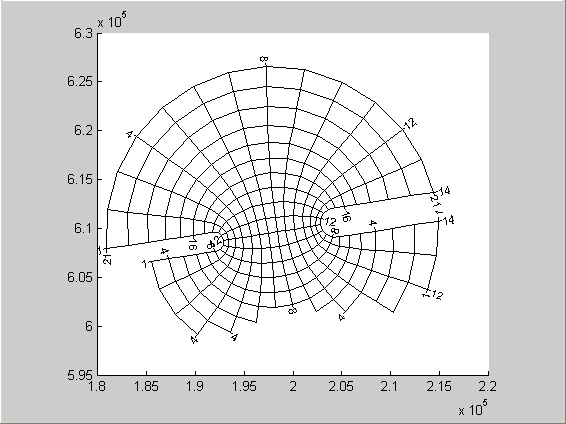
\includegraphics[width=100mm]{matlab/3-1.png}}
\caption{Grid layout from the Friesian Tidal Inlet model.}
\label{fig:3-1}
\end{figure}

\section{Plot thin dams: \command{thindam}}

\subsection*{Purpose}
Plot dams, weirs and vanes.

\subsection*{Syntax}
\begin{Verbatim}
thindam(NFStruct, T)
thindam(NFStruct, T, '3D')
thindam(XCOR, YCOR, UDAM, VDAM)
thindam('xyw', XDAM, YDAM, WDAM)
thindam(..., 'PropertyName', PropertyValue)
H = thindam(...)
[X, Y] = thindam(...)
[X, Y, M, N] = thindam(...)
[X, Y, Z] = thindam(...)
[X, Y, BOTTOM, TOP] = thindam(...)
[X, Y, BOTTOM, TOP, M, N] = thindam(...)
\end{Verbatim}

\subsection*{Description}
\command{thindam(NFStruct,T)} plots the KFU/V (drying/flooding) dams for time step T if T>0.
It plots the KCU/V thin dams if T==0 (default if T is not specified).
The function supports \file{trim-*} and \file{com-*} files.

\command{thindam(NFStruct, T, '3D')} same as above but now the dams will be plotted as 3D surfaces based on the bottom and water level information in the specified NEFIS file, \file{trim-*} or \file{com-*} file.

\command{thindam(XCOR, YCOR, UDAM, VDAM)} plots the specified U and V dams on the specified grid.
The XCOR and YCOR represent the bottom points.
Valid entries for UDAM and VDAM are:
\begin{itemize}
\item matrix of same size as XCOR/YCOR with a 1 representing a dam and a 0 indicating no dam.
\item D x 2 matrix specifying the N, M co-ordinates of the dams
\item D x 4 matrix specifying the begin/end N, M co-ordinates of the dams like in the Delft3D input files.
\end{itemize}

\command{thindam('xyw', XDAM, YDAM, WDAM, ...)} plots dams with their centre at specified (XDAM, YDAM) locations with specified width/length WDAM.
This function is useful for non-grid oriented dams.

A 3D effect can be added to these user-specified dams by specifying bottom and top levels using \command{thindam(..., 'bottom', <bottom\_args>, 'top', <top\_args>)}.
It plots the dams as 3D surfaces with specified top and bottom elevations.
The elevation data should be specified with positive direction up.
Additional supported options are:

\begin{itemize}
\item \command{'angle', <angle\_args>}
The dams/vanes are rotated to match the specified angle in degrees with respect to the positive X-axis  (positive angle in anti-clockwise direction).
\item \command{'color', <color\_args>}
The dams are coloured using the specified data.
\item \command{'thickness', <thickness\_args>}
The thickness of the dams is specified (default 0).
\end{itemize}

Valid entries for all options are:
\begin{itemize}
\item a constant, uniform value for all dams
\item a matrix of same size as XCOR/YCOR containing data in the depth points.
\item a matrix of same size as XCOR/YCOR containing data in the water level points.
To distinguish this entry from the former you need to add the string 'H' or 'S' as an extra argument after the matrix.
For example \command{thindam(..., 'top', ELEVMATRIX, 'H', ...)} indicates that the top level of the dams are derived from the specified data in water level points (the value will be used uniformly along each elementary dam).
\item two matrices of same size as XCOR/YCOR containing data in the U and V points.
\item two D x s arrays specifying the property of the individual dams.
If the array is D x 1 the value is constant along each elementary dam.
If the array is D x 2 the first value is taken for the dam end with lowest (N,M) while the second elevation for the dam end with highest (N,M).
The first array specifies the elevation for dams in U direction the second array for dams in the V direction.
For example \command{thindam(..., 'top', ELEVU, ELEVV, ...)}.
This option cannot be used in combination with option 1 for the UDAM and VDAM entries.
The number of values should match the number of dam records/elementary dams.
\end{itemize}

If a colour data field has been specified, there are a few more options available:

\begin{itemize}
\item \command{'shape',<type>} \\
The dam shape: 'dam' (default) or 'rhombus'.
\item \command{'drawdams',<onoff>}\\
Flag to draw dams.
Can be set to 'on' (default) or 'off'.
\item \command{'drawlabels',<onoff>}\\
Flag to draw the colour values as text labels.
Can be set to 'on' or 'off' (default).
\item \command{'labelformat',<format>}\\
Defines the format for displaying the values (default '\%g')
\item \command{'fontsize',<size>}\\
Defines the size of the labels.
\end{itemize}

If the 'xyw' syntax is used, then valid entries for the options are
\begin{itemize}
\item a constant (uniform value for all dams), and
\item a matrix of same size as XDAM/YDAM/WDAM.
\end{itemize}

\command{H = thindam(...)} returns the handle of the line/surface object used for plotting the dams.

\command{[X, Y] = thindam(...)} returns the x,y-arrays normally used for plotting.
The dams are not plotted.
This syntax is only valid if the input arguments indicate a 2D dam plot.

\command{[X, Y, M, N] = thindam(...)} returns four nx2 matrices containing per row a pair of end points for an elementary dam (X and Y co-ordinates, M and N index).
This syntax is only valid if the input arguments indicate a 2D dam plot.

\command{[X, Y, Z] = thindam(...)} returns the x,y,z-arrays normally used for plotting.
The dams are not plotted.
This syntax is only valid if the input arguments indicate a 3D dam plot.

\command{[X, Y, BOTTOM, TOP] = thindam(...)} returns four nx2 matrices containing per row a pair of end points for an elementary dam: X co-ordinates, Y co-ordinates, bottom elevation and top elevation.
This syntax is only valid if the input arguments indicate a 3D dam plot.

\command{[X, Y, BOTTOM, TOP, M, N] = thindam(...)} returns six nx2 matrices containing per row a pair of end points for an elementary dam: X co-ordinates, Y co-ordinates, bottom elevation, top elevation, M index, N index.
This syntax is only valid if the input arguments indicate a 3D dam plot.

\subsection*{Example, \Fref{fig:3-2}}
\begin{Verbatim}
>> vs_use D:\wl\delft3d\tutorial\wave\Siu-Lam\Com-siu
>> drawgrid('color','g')
>> set(gca,'DataAspectRatio',[1 1 1])
>> thindam(1)
>> l=thindam; set(l,'color','r')
\end{Verbatim}

\begin{figure}
\center{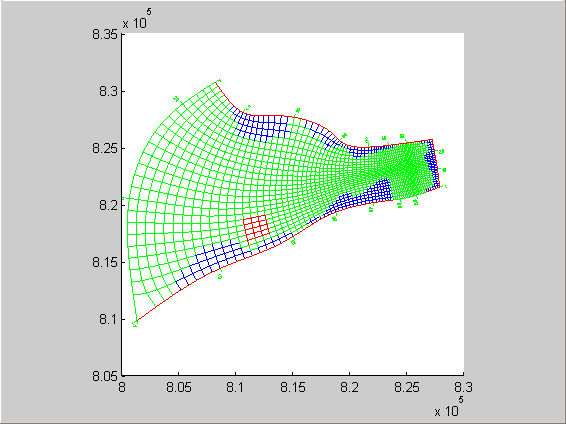
\includegraphics[width=100mm]{matlab/3-2.png}}
\caption{Example of grid and thin dams.}
\label{fig:3-2}
\end{figure}

\section{Read/write restart file: \command{trirst}}

\subsection*{Purpose}
Read/write \DFLOW\ restart file.

\subsection*{Syntax}
\begin{Verbatim}
[H, U, V, ...] = trirst('read', FILENAME, SIZE)
[H, U, V, ...] = trirst('read', FILENAME, GRID)
[H, U, V, ...] = trirst('read', FILENAME, GRID, NLAYERS)
trirst('write', FILENAME, H, U, V, ...)
trirst('write', FILENAME, PLATFORM, H, U, V, ...)
\end{Verbatim}

\subsection*{Description}
\command{[H, U, V, ...] = trirst('read', FILENAME, SIZE)} and
\command{[H, U, V, ...] = trirst('read', FILENAME, GRID)} where GRID was read in from the \file{$\ast$.grd} file by WLGRID read data from a \DFLOW\ restart file of a 2D simulation.
The dimensions of the underlying grid must be specified.
This can be done either by manually specifying the grid size as [M N], or by automatic derivation from a grid.

\command{[H, U, V, ...] = trirst('read', FILENAME, GRID, NLAYERS)} reads data from a \DFLOW\ restart file of a 3D simulation.
The NLAYERS arrays indicate the number of layers used for the various variables.
In the example syntax: \command{NLAYERS = [NLAYERH, NLAYERU, NLAYERV, ...]}.

\command{trirst('write', FILENAME, H, U, V, ...)} writes the specified matrices to the indicated restart file.
Because the restart file is stored in a platform dependent manner, care should be taken to write the appropriate type of restart file.
By default the routine writes the data in the format compatible with the computer on which MATLAB is running.
A different platform can be chosen by using the following syntax:
\command{trirst('write', FILENAME, PLATFORM, H, U, V, ...)}
where PLATFORM can be 'pc' or 'unix'.
Both Windows and Linux versions of Delft3D use the byte order indicated by 'pc'.

\section{Read/write depth file: \command{wldep}}

\subsection*{Purpose}
Read/write Delft3D field files (e.g. depth files).

\subsection*{Syntax}
\begin{Verbatim}
DEPTH = wldep('read', FILENAME, SIZE)
DEPTH = wldep('read', FILENAME, GRID)
STRUCT = wldep(..., 'multiple')
[FLD1, FLD2, ...] = wldep(..., 'multiple')
wldep('write', FILENAME, MATRIX)
\end{Verbatim}

\subsection*{Description}
\command{wldep} can be used to read and write Delft3D field files used for specifying depth and roughness data.

\command{DEPTH = wldep('read', FILENAME, SIZE)} or \command{DEPTH = wldep('read', FILENAME, GRID)} where the dimensions [M N] of the data is either user-specified or derived from the GRID data set that was obtained from \command{wlgrid}.
\command{STRUCT = wldep(..., 'multiple')} to read multiple fields from the file (e.g. in case of a roughness file).
The function returns a structure vector with one field: Data.
Use \command{[FLD1, FLD2, ...] = wldep(..., 'multiple')} to read multiple fields from the file and store the result in separate output arguments.

Use \command{wldep('write', FILENAME, MATRIX)} or \command{wldep('write', FILENAME, STRUCT)} to write data to a \file{$\ast$.dep} file.
Multiple data sets can be written by specifying a structure vector STRUCT with one field data.

\subsection*{Example, \Fref{fig:3-3}}
\begin{Verbatim}
>> G=wlgrid('read','D:\wl\delft3d\tutorial\mor\ymu\r1-nri.grd');
Warning: Grid enclosure not found.
>> D=wldep('read','D:\wl\delft3d\tutorial\mor\ymu\r1-nri.dep',G);
>> surf(G.X,G.Y,-D(1:end-1,1:end-1));
>> shading flat
>> view(-60,30)
>> set(gca,'da',[1 1 1/300])
>> camlight
\end{Verbatim}

\begin{figure}
\center{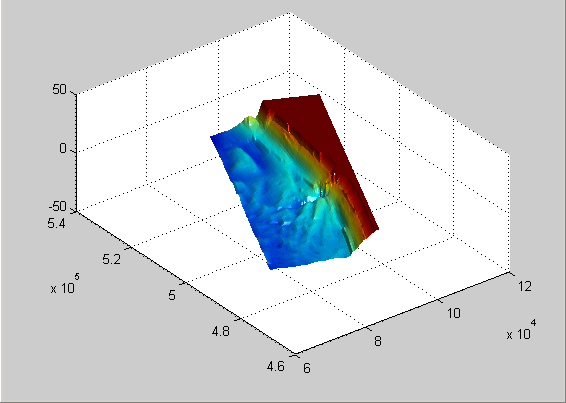
\includegraphics[width=100mm]{matlab/3-3.png}}
\caption{Example of 3D depth plot.}
\label{fig:3-3}
\end{figure}

\section{Read/write grid file: \command{wlgrid}}

\subsection*{Purpose}
Read/write a \DFLOW\ grid file.

\subsection*{Syntax}
\begin{Verbatim}
[X,Y,ENC] = wlgrid('read', FILENAME)
GRID = wlgrid('read', FILENAME)
OK = wlgrid('write', FILENAME, X, Y, ENC)
\end{Verbatim}

\subsection*{Description}
\command{[X, Y, ENC] = wlgrid('read', FILENAME)} reads the grid and enclosure from the Delft3D \file{$\ast$.grd} and \file{$\ast$.enc} files.
X, Y, and enclosure are returned as separate output arguments.
\command{GRID = wlgrid('read', FILENAME)} returns a structure with X, Y, and Enclosure fields.

\command{OK = wlgrid('write', FILENAME, X, Y, ENC)} writes the GRID to \file{$\ast$.grd} and \file{$\ast$.enc} files that can be used by Delft3D.
If the last argument (ENC) is not specified, the enclosure file is not written.

\section{Read/plot velocity field: \command{xyveloc}}

\subsection*{Purpose}
Read velocity data from a \file{trim-*} or \file{com-*} file.

\subsection*{Syntax}
\begin{Verbatim}
[U, V] = xyveloc(NFStruct, TimeStep)
[U, V, W] = xyveloc(NFStruct, Index)
[X, Y, U, V] = xyveloc(NFStruct, TimeStep)
[X, Y, Z, U, V, W] = xyveloc(NFStruct, Index)
[...] = xyveloc(..., 'option')
\end{Verbatim}

\subsection*{Description}
\command{[U, V] = xyveloc(NFStruct, TimeStep)} reads the velocity field at the specified time step from the specified NEFIS file.
By default TimeStep is the last field of the CURTIM or map-series group.
The default NEFIS file is the last opened NEFIS file.

\command{[X, Y, U, V] = xyveloc(NFStruct, TimeStep)} returns not only the velocities, but also the co-ordinates of the grid points at which the velocities are given (water level points).

\command{[U, V, W] = xyveloc(NFStruct, Index)} reads a 3D velocity field (x,y,z components).
\command{[X, Y, Z, U, V, W] = xyveloc(NFStruct, Index)} reads the 3D velocity field (x,y,z components) and returns the 3D co-ordinates of the velocity values.

\command{[...] = XYVELOC(..., 'option')} where the string 'option' equals

\begin{itemize}
\item 'vort': computes the z-component of the vorticity.
Only one output argument is required in this case.
\item 'total', 'fluc', 'mean': reads the total velocity, fluctuation component, or mean velocity field in case of an HLES simulation (trim-file, 2D only).
The default setting is 'total'.
\end{itemize}


\subsection*{Example, \Fref{fig:3-4}}
\begin{Verbatim}
>> vs_use D:\wl\delft3d\tutorial\wave\Siu-Lam\Com-siu
>> [x,y,u,v]=xyveloc;
>> quiver(x,y,u,v)
>> drawgrid('color','g')
>> set(gca,'da',[1 1 1])
>> hold on
>> quiver(x,y,u,v)
\end{Verbatim}

\begin{figure}
\center{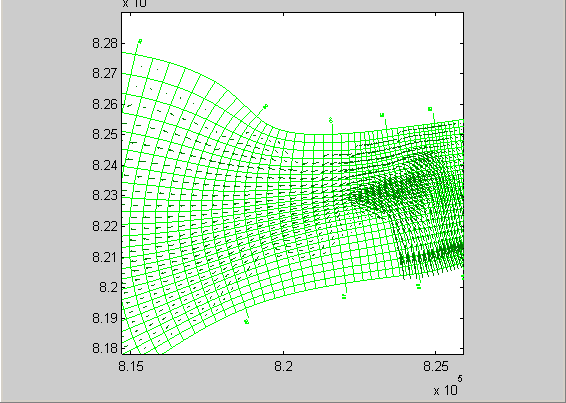
\includegraphics[width=100mm]{matlab/3-4.png}}
\caption{Example of vector velocity plot.}
\label{fig:3-4}
\end{figure}

\section{Generic read data: \command{qpread}}

\subsection*{Purpose}
Get information/data from a data file.
Provides access to the functionality of the QUICKPLOT interface.

\subsection*{Syntax}
\begin{Verbatim}
[DataFields, Dims, NVal] = qpread(FileInfo)
DataProps = qpread(FileInfo)
Size    = qpread(FileInfo, DataProp, 'size')
Size    = qpread(FileInfo, DataFld, 'size')
Times   = qpread(FileInfo, DataProp, 'times')
Times   = qpread(FileInfo, DataFld, 'times')
StNames = qpread(FileInfo, DataProp, 'stations')
StNames = qpread(FileInfo, DataFld, 'stations')
Data    = qpread(FileInfo, DataProp, 'data', t, station, m, n, k)
Data    = qpread(FileInfo, DataFld, 'data', t, station, m, n, k)
Data    = qpread(FileInfo, DataProp, 'griddata', t, station, m, n, k)
Data    = qpread(FileInfo, DataFld, 'griddata', t, station, m, n, k)
\end{Verbatim}

\subsection*{Description}
The \command{qpread} function supports reading data from various data files.
Which data sets can be read from a specific data file can be obtained from the function by one of the following two commands:

\command{[DataFields, Dims, NVal] = qpread(FileInfo)} returns the data fields available from the data file specified using the FileInfo structure.
An acceptable FileInfo can be obtained from any of the following three commands: \command{qpfopen}, \command{qpfile}, \vsuse.
If FileInfo is not specified the last opened NEFIS file is used (same condition applies to the other calls to \command{qpread}).
The variable DataFields is a cell array of strings containing the names of the data sets in the file.
The variable Dims indicates relevant dimensions for the data fields:

\begin{tabular}{ll}
First column of Dims:  & Time step \\
Second column of Dims: & Station name \\
Third column of Dims:  & M \\
Fourth column of Dims: & N \\
Fifth column of Dims:  & K \\
\end{tabular}

NVal equals one for scalar data sets, 2 (or 3) for vector data sets.

\command{DataProps = qpread(FileInfo)} returns a structure containing fields with the above mentioned data and some extra information for internal use by the \command{qpread} and \command{d3d\_qp} functions.

Based on the information returned by either one of these two \command{qpread} statements you may select a data field.
This data field can be identified using its name provided in the DataFields cell array (DataFields{i}) or its record in the DataProps structure (DataProps(i)).
For each data field you can obtain more information by subsequent calls to \command{qpread}.

\begin{Remark}
\item You should not request data for the separator fields with name \command{'-----'}.
\end{Remark}

\command{Size = qpread(FileInfo, DataProp/DataFldName, 'size')} returns a 1 x 5 array containing the maximum size of the five dimensions mentioned above.
The second parameter can be either a string (data field name) or a record from the DataProps structure.
The latter is necessary if the data field name is not unique.

\command{Times = qpread(FileInfo, DataProp/DataFldName, 'times')} returns an array of the times for the specified data field if relevant.

\command{StNames = qpread(FileInfo, DataProp/DataFldName, 'stations')} returns an array of the station names for the specified data field if relevant.

\command{Data = qpread(FileInfo, DataProp/DataFld, 'data', t, station, m, n, k)} returns the data for the specified data field at the indicated time steps, specified station, and M, N, K co-ordinates.
Only those parameters should be specified that have non-zero dimension in Dims and Size.
For a data field at a station often only time and station.
For spatial data sets not the station but a selection of M, N and K.
Following restrictions apply to the retrieval of the data

\begin{itemize}
\item station: index of the station in the StNames array (scalar).
\item 0 (all points) or scalar value (m index).
\item 0 (all points) or scalar value (n index).
\item 0 (all points) or scalar value (k index).
\end{itemize}

\command{Data = qpread(FileInfo, DataProp, 'griddata', t, station, m, n, k)} returns the data and grid for the specified data field at the indicated time steps, specified station, and M, N, K co-ordinates.
In both cases the output argument Data is a structure containing a Time field.
If the data is scalar, the data is returned in the Val field.
If the data is vector data, it is returned as Xcomp and Ycomp fields.

\subsection*{Example, \Fref{fig:3-5}}
\begin{Verbatim}
>> F=qpfopen('D:\wl\delft3d\tutorial\gpp\trim-edw.dat');
>> I=qpread(F);
>> I(9)

ans =

          Name: 'water level'
       DimFlag: [1 0 1 1 0]
    DataInCell: 1
          NVal: 1
       VecType: ''
           Loc: 'z'
        ReqLoc: 'z'
         Loc3D: ''
         Group: 'map-series'
          Val1: 'S1'
          Val2: ''
        SubFld: []
           MNK: 0

>> S=qpread(F,I(9),'griddata')

S =

       X: [87x227 double]
       Y: [87x227 double]
     Val: [87x227 double]
    Time: 7.2942e+005

>> contour(S.X,S.Y,S.Val,50)
>> view(90,90)
>> set(gca,'da',[1 1 100])
\end{Verbatim}

\begin{figure}
\center{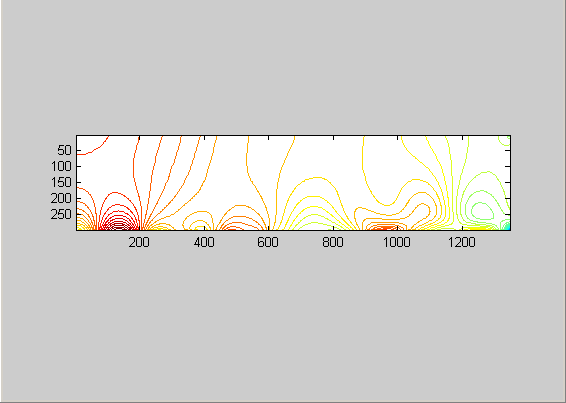
\includegraphics[width=100mm]{matlab/3-5.png}}
\caption{Example of contour plot.}
\label{fig:3-5}
\end{figure}

\section{Generic open file: \command{qpfopen}}

\subsection*{Purpose}
Opening a data file.
Provides access to the functionality of the QUICKPLOT interface.

\subsection*{Syntax}
\begin{Verbatim}
FileInfo=qpfopen('Filename')
FileInfo=qpfopen('DataFile','GridFile')
FileInfo=qpfopen
\end{Verbatim}

\subsection*{Description}
The \command{qpfopen} functions can be used to open all data files that QUICKPLOT can open (see the appendix of the QUICKPLOT manual for an overview of all file formats).

\command{FileInfo=qpfopen('Filename')} opens the specified output file and returns a structure containing data used by the \command{qpread} function.

For WAQ or PART \file{$\ast$.map} files you should also specify an \file{$\ast$.lga} grid file: \command{FileInfo = qpfopen('DataFile', 'GridFile')}
If no grid file is specified then the map file is treated as a history file with an observation point at each location.

\command{FileInfo=qpfopen}
When no arguments are passed to the function, you are asked to specify the file using a standard file selection dialog window.
If you try to open a WAQ or PART \file{$\ast$.map} file, the function asks for the additional grid file.

\section{Get file opened by QUICKPLOT: \command{qpfile}}

\subsection*{Purpose}
Get information about the currently selected file in QUICKPLOT.
Provides access to the functionality of the QUICKPLOT interface.

\subsection*{Syntax}
\begin{Verbatim}
FileInfo=qpfile
\end{Verbatim}

\subsection*{Description}
To make switching between the user interface of QUICKPLOT and MATLAB's command line easier, the \command{qpfile} function provides easy access to the currently selected file in the QUICKPLOT interface.

\command{FileInfo=qpfile} returns the structure of the data file selected in the QUICKPLOT interface.
